% begin module sequence-ex6
\begin{frame}
\begin{example}[Example 6, p. 715]
Is the sequence $a_n = (-1)^n$ convergent or divergent?
\begin{columns}[c]
\column{.5\textwidth}
\ \only<handout:0| -1>{%
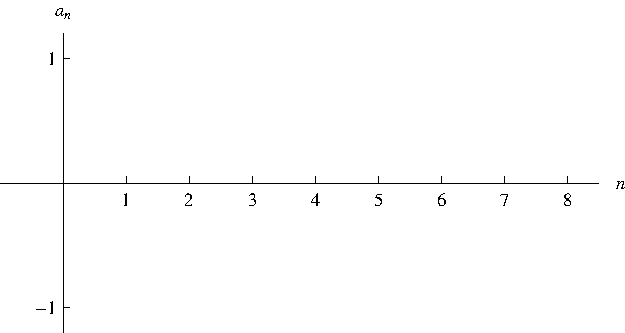
\includegraphics[width=6cm]{sequences/pictures/12-01-ex6a.pdf}%
}%
\only<2->{%
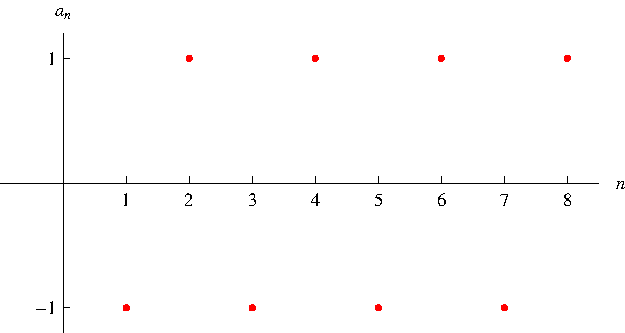
\includegraphics[width=6cm]{sequences/pictures/12-01-ex6b.pdf}%
}%
\column{.5\textwidth}
\begin{itemize}
\item<2->  The terms oscillate between $-1$ and $1$ infinitely many times.
\item<3->  Therefore the sequence doesn't approach any number.
\item<4->  $\{ a_n\}$ is divergent.
\end{itemize}
\end{columns}
\end{example}
\end{frame}
% end module sequence-ex6
